\documentclass[a4paper]{article}
\usepackage{lipsum}
\usepackage{url}
\usepackage{graphicx}
\usepackage{indentfirst}
\usepackage{xcolor}
\usepackage[margin=2cm]{geometry}
\graphicspath{ {images/} }

%Custom Commands
\newcommand{\Pokemon}{Pok\'{e}mon}

%NOTE: 2,000 Words / 4 Pages
%TODO: Also need to do ethics checklist
%TODO: Get a better font and layout :P
%TODO: Think of a better title?
%NOTE: Make the Work Plan codes more detailed
%TODO: Rewrite the Work Plan Descriptions
%TODO: Make sure work plan description titles follow a sensible structure and match
%TODO: Add installing and playing with framework to work plan

\begin{document}

%Title Information
\title{
    Project Proposal
    \\ \large{G54IRP/COMP4027}
    \\ \large{Project Title: AI for General Video Game Playing}\vspace{-3ex}}
\author{4262648 Benjamin Charlton (psybc3)}
\date{\vspace{-2ex}12\textsuperscript{th} October 2017}
\maketitle

\section{Background and Motivation}
NB:  Currently this section isn't complete as I have been doing background research to better understand what would be relevant to put in this section.
\par
\pagebreak

\section{Aims and Objectives}
This research projects sets out to create and implement a General AI to play video games.
To test and evaluate this goal the solution developed will be tested against the GVGAI framework using the competition rules.\cite{GVGAI2014}
The project will produce an AI to play in the GVGAI framework as well as a research paper describing the performance of the AI created.
\bigbreak
\noindent The objectives of this project are:
\begin{description}
    \item [Background Research]
    Perform research into the current state of AI game playing, general AI, and current well performing solutions to the GVGAI competition.
    The result of this background study will be used to direct the rest of the project and determine a suitable method to tackle the problem with.

    \item [Design a General AI]
    Design an AI suitable to playing general video games as presented in the GVGAI framework.
    The design and approach will be heavily influenced by the research performed earlier in the project, taking account of other previous methods both in and out of the general game playing field as well as how the problem is presented in the framework.

    \item [Develop a General AI]
    Implement and develop the design created to tackle the problem.
    This will be the primary output of the project.
Due to the heavy reliance on the background research it isn't clear what this stage will involve.

    \item [Evaluation and Analysis of Solution]
    Compare and analyse the performance of the solution against the other entries to the GVGAI competition and potentially against human players.
    If the solution performs well there may be the ability to test them in unseen environments, such as Video Games that aren't shown in the training sets.
\end{description}

\section{Work Plan}
To help outline the project flow and I have created a gantt chart (found in the appendix) and the following descriptions of each portion.
Some parts of the work plan (specifically development) are currently very vague as the initial research needs to happen to acquire the knowledge and insight of how to proceed.
\par
The work plan will be updated to break down these tasks in to more concrete steps with accurate timeframes once the direction of the project is better known.
Updates to the work plan will also come to better reflect how long certain parts of the project will take if adjustments need to be made.

%Explanations of all of the Points on the work plan
\begin{description}
\item [\large{Documentation}]
\item [D1 - Project Proposal Draft]
Write the project proposal draft for approval and feedback from supervisor, due 12\textsuperscript{th} October.
\item [D2 - Project Proposal]
Any revisions to the project proposal that need to be made after supervisor feedback, due 22\textsuperscript{rd} October.
\item [D3 - Preliminary Ethics Checklist]
Fill out and submit the preliminary ethics checklist, no further ethical checks should be required so no further time is scheduled.
\item [D4 - Interim Report Outline Sections]
Create a basic outline of how the interim report will look with respect to the sections included and their content
\item [D5 - Interim Report Related Work]
Write the related work section of the interim report, discussing previous research in General AI and game playing. This will happen alongside the research steps that correspond to this task.
\item [D6 - Interim Report Draft]
Create a draft of the interim report with all sections roughly finished.
\item [D7 - Interim Report Finalise]
Add the finishing touches to the interim report summarising the work so far, due 7\textsuperscript{th} December.
\item [D8 - Research Paper]
Write the final research paper, due 12\textsuperscript{th} April.
\colorbox{yellow}{NB: Want to break this down into further sub tasks}

\item [\large{Research}]
\item [R1 - Project Proposal Research]
Background research into the problem and history of the field for the Background section of the project proposal, as well as research into the module structure to help plan out the project.
\item [R2 - GVGAI Basic Research]
Basic research into the structure and aims of the GVGAI competition.
\item [R3 - GVGAI Papers for Related Works]
Background research into previous attempts at the GVGAI competition, looking into successful methods and analysis of the problem to better formulate a new approach to the problem.
\item [R4 - Other Related Works]
Background research into further related works to the problem, looking into AI game playing and general AI problem solving.

\item [\large{Development}]
\item [S1 - Develop Solution]
Currently vague as the sub tasks involved in this step will depend on the method chosen to tackle the problem.

\item [\large{Presentation}]
\item [P1 - Presentation General Outline]
Begin work on the presentation outlining the general content and flow.
\item [P3 - Create Demo for Presentation]
Create a demo of the project to show how it performs.
\item [P3 - Finalise Presentation]
Make final adjustments to the presentation and practice delivering it in its final form.
\item [P4 - Present Presentation]
Present the presentation and demo during the demo day.

\item [\large{Miscellaneous}]
\item [M1 - Create Git repository]
Create a Git repository on the School of Computer Science Git server to allow for management of the code and documentation.
\item [M3 - Install LaTeX]
Install LaTeX and any other dependencies to allow production of documentation through out the project.
\item [M3 - SET/SEM Questionaries]
Module feedback to be completed. Student Evaluation of Teaching and Student Evaluation of Modules to comment upon supervisor teaching and the module as a whole respectively.

\item [\large{Other Commitments}]
\item [C1 - Welcome Weeks]
First weeks of the academic year, time set aside to allow for settling in as well as running various welcome events.
\item [C2 - Christmas Holiday]
Time off after Autumn term, Partially set aside to all for a break and time to relax..
\item [C3 - Autumn Exams]
Potentially could have exams during the entire 2 weeks so is set aside to allow for revision and the exams themselves.
This can be updated to give a better reflection of when exams will be at a later date.
\item [C4 - Easter Holiday]
Time off after Spring term, As no teaching is happening will give more time to concentrate on coursework and the presentation.
\end{description}

\section{Appendix}
%Bibliography
\bibliography{ProjectProposal}
\bibliographystyle{plain}

%Work Plan
\clearpage
\begin{center}
    \Large{Work Plan}\\
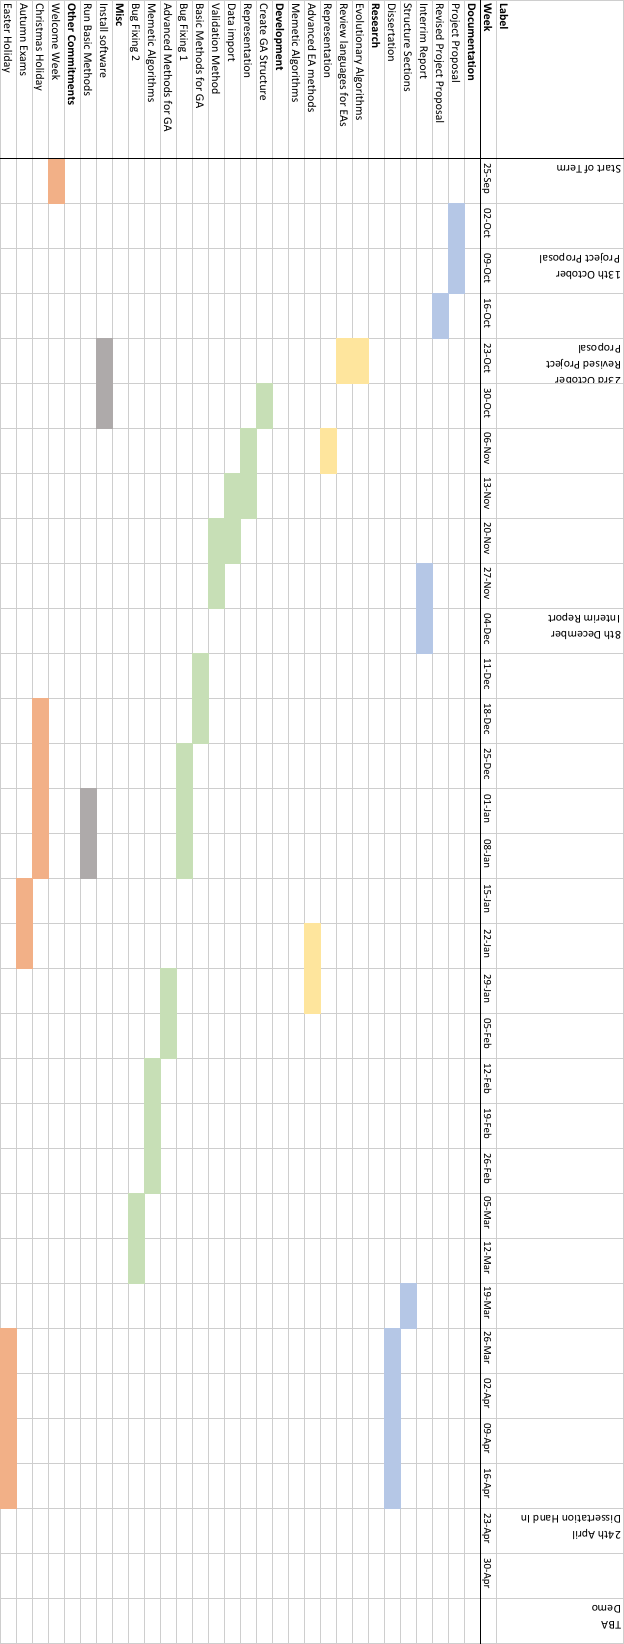
\includegraphics[height=24.8cm]{workPlan.png}
\end{center}


\end{document}
